%%% LaTeX Template: Two column article
%%%
%%% Source: http://www.howtotex.com/
%%% Feel free to distribute this template, but please keep to referal to http://www.howtotex.com/ here.
%%% Date: February 2011

%%% Preamble
\documentclass[	DIV=calc,%
							paper=a4,%
							fontsize=12pt,%
							onecolumn]{scrartcl}	 					% KOMA-article class

\usepackage{lipsum}													% Package to create dummy text
\usepackage[brazil]{babel}										% English language/hyphenation
\usepackage[protrusion=true,expansion=true]{microtype}				% Better typography
\usepackage{amsmath,amsfonts,amsthm}					% Math packages
\usepackage[pdftex]{graphicx}									% Enable pdflatex
\usepackage[svgnames]{xcolor}									% Enabling colors by their 'svgnames'
\usepackage[hang, small,labelfont=bf,up,textfont=it,up]{caption}	% Custom captions under/above floats
\usepackage{epstopdf}												% Converts .eps to .pdf
\usepackage{subfig}													% Subfigures
\usepackage{booktabs}												% Nicer tables
\usepackage{fix-cm}													% Custom fontsizes
\usepackage[utf8]{inputenc}
\usepackage[top=2.5cm, bottom=2.5cm, left=2.5cm, right=2.5cm]{geometry}
\usepackage[ddmmyyyy]{datetime}
\addto\captionsenglish{%
	\renewcommand\tablename{Tabela}
	\renewcommand\figurename{Figura}
} 
 

 
%%% Custom sectioning (sectsty package)
\usepackage{sectsty}													% Custom sectioning (see below)
\allsectionsfont{%															% Change font of al section commands
	\usefont{OT1}{phv}{b}{n}%										% bch-b-n: CharterBT-Bold font
	}

\sectionfont{%																% Change font of \section command
	\usefont{OT1}{phv}{b}{n}%										% bch-b-n: CharterBT-Bold font
	}



%%% Headers and footers
\usepackage{fancyhdr}												% Needed to define custom headers/footers
	\pagestyle{fancy}														% Enabling the custom headers/footers
\usepackage{lastpage}	

% Header (empty)
\lhead{}
\chead{}
\rhead{}
% Footer (you may change this to your own needs)

%% ====================================
%% ====================================
%% mude o rodape  do projeto
%% ====================================
%% ====================================

\lfoot{\footnotesize \texttt{Template para entrega de texto} \textbullet ~Modelo de projeto}


\cfoot{}
\rfoot{\footnotesize página \thepage\ de \pageref{LastPage}}	% "Page 1 of 2"
\renewcommand{\headrulewidth}{0.0pt}
\renewcommand{\footrulewidth}{0.4pt}



%%% Creating an initial of the very first character of the content
\usepackage{lettrine}
\newcommand{\initial}[1]{%
     \lettrine[lines=3,lhang=0.3,nindent=0em]{
     				\color{DarkGoldenrod}
     				{\textsf{#1}}}{}}



%%% Title, author and date metadata
\usepackage{titling}															% For custom titles

\newcommand{\HorRule}{\color{DarkGoldenrod}%			% Creating a horizontal rule
									  	\rule{\linewidth}{1pt}%
										}

\pretitle{\vspace{-30pt} \begin{flushleft} \HorRule 
				\fontsize{50}{50} \usefont{OT1}{phv}{b}{n} \color{DarkRed} \selectfont 
				}

%% ====================================
%% ====================================
%% mude o titulo  do projeto
%% ====================================
%% ====================================

\title{Modelo incremental adaptado }					% Title of your article goes here

%% ====================================



\posttitle{\par\end{flushleft}\vskip 0.5em}

\preauthor{\begin{flushleft}
					\large \lineskip 0.5em \usefont{OT1}{phv}{b}{sl} \color{DarkRed}}
\author{Erik Henrique de Oliveira, Vitor Padiar Carnevalli, João Pirolo }  	% Author name goes here


\postauthor{\footnotesize \usefont{OT1}{phv}{m}{sl} \color{Black} 
					\\Universidade Tecnológica Federal do Paraná - Câmpus Cornélio Procópio 								% Institution of author
					\par\end{flushleft}\HorRule}

\date{}																				% No date




%%% Begin document
\begin{document}
\maketitle
\thispagestyle{fancy} 	
\thispagestyle{empty}		% Enabling the custom headers/footers for the first page 
% The first character should be within \initial{}




%% ====================================
%% ====================================
%% mude o resumo  do projeto
%% ====================================
%% ====================================
\initial{E}\textbf{ste trabalho apresenta uma daptação dos processos incremental e unificado, onde um grupo de três Eng. de Software trabalhão no processo de desenvolvimento de um produto comercial de software. } 

%% ====================================
\begin{figure}
	\centering
	
\includegraphics{utfpr}
\end{figure}

\vspace{3cm}
\centerline{\textit{\textbf{\today}}}

\clearpage
    \renewcommand*\listfigurename{Lista de figuras}
\listoffigures

\renewcommand*\listtablename{Lista de tabelas}
\listoftables




\clearpage
\renewcommand{\contentsname}{Sumário}
\tableofcontents
\clearpage

%% ====================================
%% ====================================
%% Inicio do texto
%% ====================================
%% ====================================
\section{Introdução}

O desenvolvimento de um software é uma grande tarefa que pode ser estendida por vários meses, possivelmente até um ano ou mais. Para tornar esta tarefa mais rapida e pratica é importate, dividir o trabalho em partes menores ou iterações. Cada iteração resultará num incremento ou uma versão de software. 

 Iterações são passos do e incrementos são crescimentos do produto.

O princípio do processo incremental e iterativo é que, a equipe envolvida, possa refinar e aumentar,  aos pouco, a qualidade, os requisitos até atingir o sistema final.  Isso faz toda a diferença, quando falamos em grandes sistemas, a serem automatizados.   

Como o processo teve de ser adaptado a um grupo pequeno ele sofreu algumas alteraçãoes principalmente na fase de construção e transição, a nomeclatura adotada para esse modelo de prcesso foi: Processo Ágil Inclemental adaptado.

O processo foi desenvolvido pelos desenvolvedores:
\begin{itemize}
{\item João Pirolo - Github: https://github.com/JoaoPirolo,
\item Erik Zambeli - gitHub: https://github.com/ErikZA, 
\item Vitor Padiar - GitHub: https://github.com/vitorpadiar.}
\end{itemize} 
\section{Processo}

 O Processo Unificado surgiu como um processo para o desenvolvimento de software orientados a objetos. É um processo iterativo e adaptativo de desenvolvimento que devido a maneira organizada e consistente permite conduzir um projeto de sua concepção a sua implantação.
 
 O PU utiliza um paradigma evolucionário paro o desenvolvimento de softwares. O ciclo de vida iterativo é baseado em versões e incrementos sucessivos a fim de integrar um sistema adequado. Em cada iteração incrementa-se um pouco mais o produto, baseando-se na experiência obtida nas iterações anteriores e no feedback do usuário. Cada iteração pode ser considerada uma nova versão do software de duração fixa, sendo que cada uma destas inclui suas próprias atividades de análise de requisitos, projeto, implementação e testes.
 
  Em cada iteração é escolhido um pequeno subconjunto de requisitos, os quais são rapidamente projetados, implementados e testados pelos usuários. Isso leva a uma realimentação rápida de requisitos baseada em dados concretos de usuários, desenvolvedores e testes, o PU prega uma atitude de aceitar a mudança e a adaptação como fatores inevitáveis e essenciais. Não se deve tentar especificar completamente o sistema em uma tacada interação só, essa idéia cria um conjunto congelado de requisitos.
 
 O resultado de cada iteração é um sistema executável,  porém incompleto. Ele não está pronto para ser colocado em produção e pode continuar nesta situação ainda por muitas iterações mais cada iteração produz um sistema com qualidade de produto final, e não somente um protótipo.
 
  Modedelo de processo unificado figura \ref{rup1}: 
 \begin{figure}
	\centering
	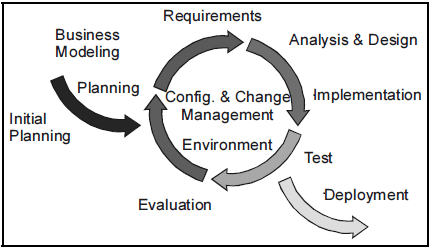
\includegraphics[]{rup1.png}
	\caption{Exemplo de Modelo Unificado}
	\label{rup1}
\end{figure}
 
 O Processo Unificado organiza suas iterações em quatro fases principais:
\begin{itemize}

\item Concepção: o objetivo desta fase é levantar, de forma genérica e pouco precisa, o escopo do projeto. Não deve existir aqui a pretensão de especificar de forma detalhada requisitos, a idéia é ter uma visão inicial do problema, estimar de forma vaga esforço e prazos e determinar se o projeto é viável e merece uma análise mais profunda.

\item Elaboração: na fase de elaboração todos (ou a grande maioria dos requisitos) são levantados em detalhes. Numa primeira iteração um ou dois requisitos, os de maior risco e valor arquitetural, são especificados em detalhes. Estes são implementados e servem como base de avaliação junto ao usuário e desenvolvedores para o planejamento da próxima iteração. Em cada nova iteração os requisitos antigos são melhor esclarecidos e novos são detalhados. Ao fim da fase, com os requisitos levantados em detalhes, os principais riscos foram tratados e pode-se então fazer estimativas mais realistas.

\item Construção: implementação iterativa dos elementos restantes de menor risco e mais fáceis e preparação para a implantação.

\item Transição: testes finais e implantação.

\end{itemize}

O Processo Unificado foi criado para ser um processo ágil de desenvolvimento e prega uma abordagem realística para a condução de um projeto. Para a sua utilização durante o desenvolvimento devido ao pequeno grupo tivemos de adaptar e modificar os atividades de suas fases para atender as necessidades do desenvolvimento.

\subsection{Papeis}

O processo original exigia a demanda de muitos papeis, para faciliar a adaptação do processo e a melhor distribuição das atividades, adotamos os seguintes papeis para nossa organização:

\begin{itemize}

	\item Gerente de Projeto: Descreve os objetivos do projeto e como ele será realizado. Inclui estimativas de custo e programação trata da identificação das atividades a serem realizadas, os artefatos e os documentos a serem produzidos,versões a serem entregues, realiza o levantamento do custo do projeto, em um segundo realise acompanha o projeto de forma constante verificando o progresso e os custos  comparando com o que foi pranejado inicialmente, elaboração de relatorios prestação de contas e de resultados.

	\item Analista de Sistema: levantamentos de requisitos e regras de negócio, mapeamento dos processos elaboração dos casos de uso basedo nos requisitos dos clientes,garantia da integridade dos sistemas, realizar o planejamento das versões, atua tambem como analista de implantação elaborando o plano de implantação da aplicação e coleta requisitos nescessarios para as proximas versões, aplica treinamento aos usuários.

	\item Desenvolvedor: Desenvolver, testar e liberar versões para a  implantação e manter o sistemas de acordo com metodologia e técnicas propostas, para garantir a qualidade, o custo e prazo.
\end{itemize} 
\subsection{Atividades}
\begin{itemize}
    

\item Atividades do Gerente Projetos tabela \ref{tab1}:
\begin{table}[h!] % coloque h! para forcar a posicao
\centering
\caption{Modifique a legenda e crie um label}
\label{tab2} %com este label vc faz referencia no texto
\begin{tabular}{|l|l|l|l|l|}
\hline
\multicolumn{1}{|c|}{\textbf{Este é um exemplo de tabela}} & \multicolumn{2}{c|}{\textbf{C1}} & \multicolumn{2}{c|}{\textbf{C2}} \\ \hline
Você pode criar a tabela no excel                          & 1              & 2               & 3               & 4              \\ \hline
Exportar para CSV                                          & 5              & 6               & 7               & 8              \\ \hline
E importar no Table Generator                              & 9              & 10              &                 &                \\ \hline
\multicolumn{5}{|c|}{\textit{Gere o tex, e adicione em seu arquivo}}                                                             \\ \hline
\end{tabular}
\end{table}

\item Atividades do Analista de Sistemas tabela \ref{tab2}:
\begin{table}[h!]
\centering
\caption{Exemplo de tabela explicativa}
\label{tab1}
\begin{tabular}{|l|l|l|}
\hline
\multicolumn{3}{|l|}{Figura na Tabela} \\ \hline
1        & Rack          & \includegraphics[scale=0.2]{fig1}        \\ \hline
2        & Rack 2        & \includegraphics[scale=0.2]{fig1}        \\ \hline
\end{tabular}
\end{table}

\item Atividades do Desenvolvedor tabela \ref{tab3}:
\begin{table}[h!]
\centering
\caption{Tabela tarefas do Desenvolvedor}
\label{tab3}
\begin{tabular}{|l|l|l|}
\hline
\begin{tabular}[c]{@{}l@{}}Item /\\  papel\end{tabular} & Desenvolvedor                                                        & Aplicações                                                                                                                                                                                                                                                                       \\\hline
1                                                       & \begin{tabular}[c]{@{}l@{}}Desenvolver\\  o código\end{tabular}      & \begin{tabular}[c]{@{}l@{}}A atividade de desenvolver incremento de software consiste \\ em escrever o código-fonte que implementa, \\ ou corrige, um ou mais requisitos do software. \\ Esta atividade pode ser \\ realizada mais de uma vez durante uma iteração.\end{tabular} \\\hline
2                                                       & \begin{tabular}[c]{@{}l@{}}Realizar teste \\ de Unidade\end{tabular} & \begin{tabular}[c]{@{}l@{}}Trata-se de um teste do tipo estrutural \\ (caixa-branca) que deve ser produzido pelo \\ programador, em parceria com o testador, antes da \\ implementação da unidade de software.\end{tabular}                                                      \\\hline
3                                                       & \begin{tabular}[c]{@{}l@{}}Corrigir \\ Bugs\end{tabular}             & \begin{tabular}[c]{@{}l@{}}Avaliar os resultados positivos \\ e negativos dos testes.\end{tabular}                                                                                                                                                                               \\\hline
4                                                       & \begin{tabular}[c]{@{}l@{}}Integração \\ do Software\end{tabular}    & \begin{tabular}[c]{@{}l@{}}desenvolver o sistema dividindo-o em módulos ou componentes, \\  funcionalidades do componente integrado devem \\ funcionar corretamente no sistema produzido.\end{tabular}                                                                           \\\hline
5                                                       & \begin{tabular}[c]{@{}l@{}}Teste de \\ Aceitação\end{tabular}        & \begin{tabular}[c]{@{}l@{}}Nesta etapa devem ser executados os testes de sistema e, \\ se aplicáveis, os testes de aceitação.\end{tabular}                                                                                                                                       \\\hline
6                                                       & \begin{tabular}[c]{@{}l@{}}Liberação \\ da Versão\end{tabular}       & \begin{tabular}[c]{@{}l@{}}Liberar uma versão testada \\ e atualizada do Incremento\end{tabular}                                                                           \\\hline                                                                                                     
\end{tabular}
\end{table}

\end{itemize}
\section{Execução do projeto}

Relacione as atividades com os integrantes, crie um cronograma conforme orientações
\subsection{Backlog e sprints}
-- item obrigatório --

Evidencie todos os stakeholders involvidos


\subsection{Estado atual}
Apresente os artefatos gerados em ordem cronológica, conforme processo.


\section{Referências bibliográficas}
Utilize o mendley, o jabref ou diretamente o bibtex para gerenciar suas referências biliográficas. As referências são criadas automaticamente de acordo com o uso no texto.

Exemplo: Redes de computadores, segundo \cite{t2013} é considerada..... Já \cite{kurose2010} apresenta uma versão...

Analisando os pressupostos de \cite{ref3} e \cite{ref4} concluimos que....


\renewcommand\refname{} %%Referências bibliográficas}  
\bibliographystyle{ieeetr}
\bibliography{referencias}  

%% ***********************************************************************
%% === remover daqui =====================================================
%% ***********************************************************************
=================================================
\section{Elementos textuais - Tabelas}

%% ***********************************************************************
%% === ate aqui    =====  ================================================
%% ***********************************************************************

\end{document}